\documentclass{article}%
\usepackage[T1]{fontenc}%
\usepackage[utf8]{inputenc}%
\usepackage{lmodern}%
\usepackage{textcomp}%
\usepackage{lastpage}%
\usepackage{authblk}%
\usepackage{graphicx}%
%
\title{Up{-}regulation of focal adhesion kinase in non{-}small cell lung cancer}%
\author{Tammy Gonzalez}%
\affil{Department of Developmental, Molecular and Chemical Biology, Tufts University School of Medicine, Boston, Massachusetts, United States of America}%
\date{01{-}01{-}2009}%
%
\begin{document}%
\normalsize%
\maketitle%
\section{Abstract}%
\label{sec:Abstract}%
The Future of Life in Digital Nature, one of the Society for Science's top science journals, recently had a very intriguing article about the importance of protein transport in organism biology. The article, presented at the Experimental Biology 2010 conference by Brehm Lacar, described how a protein transporter, called HD{-}PZ, is currently being used in pSci labs in a variety of cell biology experiments as a transporter of complex structure and function in a cell by carrier route.\newline%
HD{-}PZ is a transporter for the protein polyfilm, which is essential for the production of polysaccharides in insects and other living animals. HD{-}PZ prevents interspecies confrere transfers of polysaccharides on free{-}range pests and other insects that dont have free{-}range genetic status, said Lacar. The finding shows how HD{-}PZ transports multi{-}synthetic polysaccharides, including non{-}abnormal polysaccharides.\newline%
The paper can be read here:\newline%
Future of Life in Digital Nature, January 1, 2009, at: http://www.spiti.org/DYS\newline%
DYS is an online science publishing community for scientists with a focus on journal publishing, public communication and strategic business applications. We support scientific communication via website, email, blog, email contact lists, RSS feeds, Twitter, RSS List, Twitter Tracker, webinars, and other applications that enhance science communication worldwide.

%
\subsection{Image Analysis}%
\label{subsec:ImageAnalysis}%


\begin{figure}[h!]%
\centering%
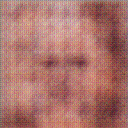
\includegraphics[width=150px]{500_fake_images/samples_5_399.png}%
\caption{A Close Up Of A Red And White Striped Tie}%
\end{figure}

%
\end{document}